\section{Praktische Aplikation \& Versuch für zu Hause (Todo : besserer Titel)}

Im Zuge der dieser Seminararbeit wurden unsere Erkenntnisse präsentiert an einer Präsentation vorgestellt. 
Dieses Thema bietet eine interessante Möglichkeit es zu visualisieren. 
Dies ist natürlich eine Wirbelringkanone. 
Damit lassen sich gezielt Wirbelringe erzeugen, um damit die Eigenschaften davon zu zeigen. 
Es gibt natürlich diverse Möglichkeiten, ein Wirbelring zu erzeugen. 
Hier zeigen wir ein Ansatz welcher möglichst einfach und nachbaubar ist.

\subsection{Bau}

\begin{figure}
\centering
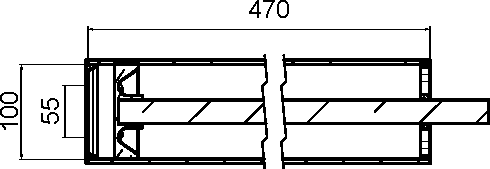
\includegraphics[width=0.8\textwidth]{papers/wirbelringe/fig/zeichnung.pdf}
\caption{Zeichnung und Masse der Wirbelringkanone \cite{Wirbelringe:3D_modelle} \label{Wirbelringe:fig:zeichnung}}
\end{figure}
Für den Bau wird ein (oder Zugang zu einem) 3D Drucker, \diameter 100 PVC Abflussrohr und eine Möglichkeit Rauch zu erzeugen, um die Wirbelringe besser zu sehen. 
Es müssen lediglich alle Teile 3D gedruckt werden (siehe \cite{Wirbelringe:3D_modelle}) und diese mit einem PVC Kleber fixiert werden. 

\subsection{Versuch}

Diese Wirbelringkanone kann nun verwendet werden, um einen Versuch durchzuführen. 
Aus Abschnitt \ref{paper:Wirbelringe:Grenzflaechen} ist bekannt, das Wirbel nur auf Grenzflächen oder sich selbst enden können. 
Um das bei einem Wirbelring aufzuzeigen, kann ein Wirbelring "gespalten" werden. 
Also ein Wirbelring soll dazu gebracht werden, die Grenzflächen von sich selbst auf etwas anderes zu wählen zum Beispiel ein Tisch. 
Mithilfe einer Kante, die wie eine Klinge funktioniert, kann der Wirbelring geschnitten werden und so umgelenkt, dass der jetzige Wirbelfaden sich weiter bewegt. 
Dieser Versuch ist in Abbildung \ref{buch:papers:Wirbelringe:fig:wirbelringversuch} dargestellt.

\begin{figure}
    \centering
    \subfigure[\label{Wirbelringe:fig:versuch_moment_1}]{
        %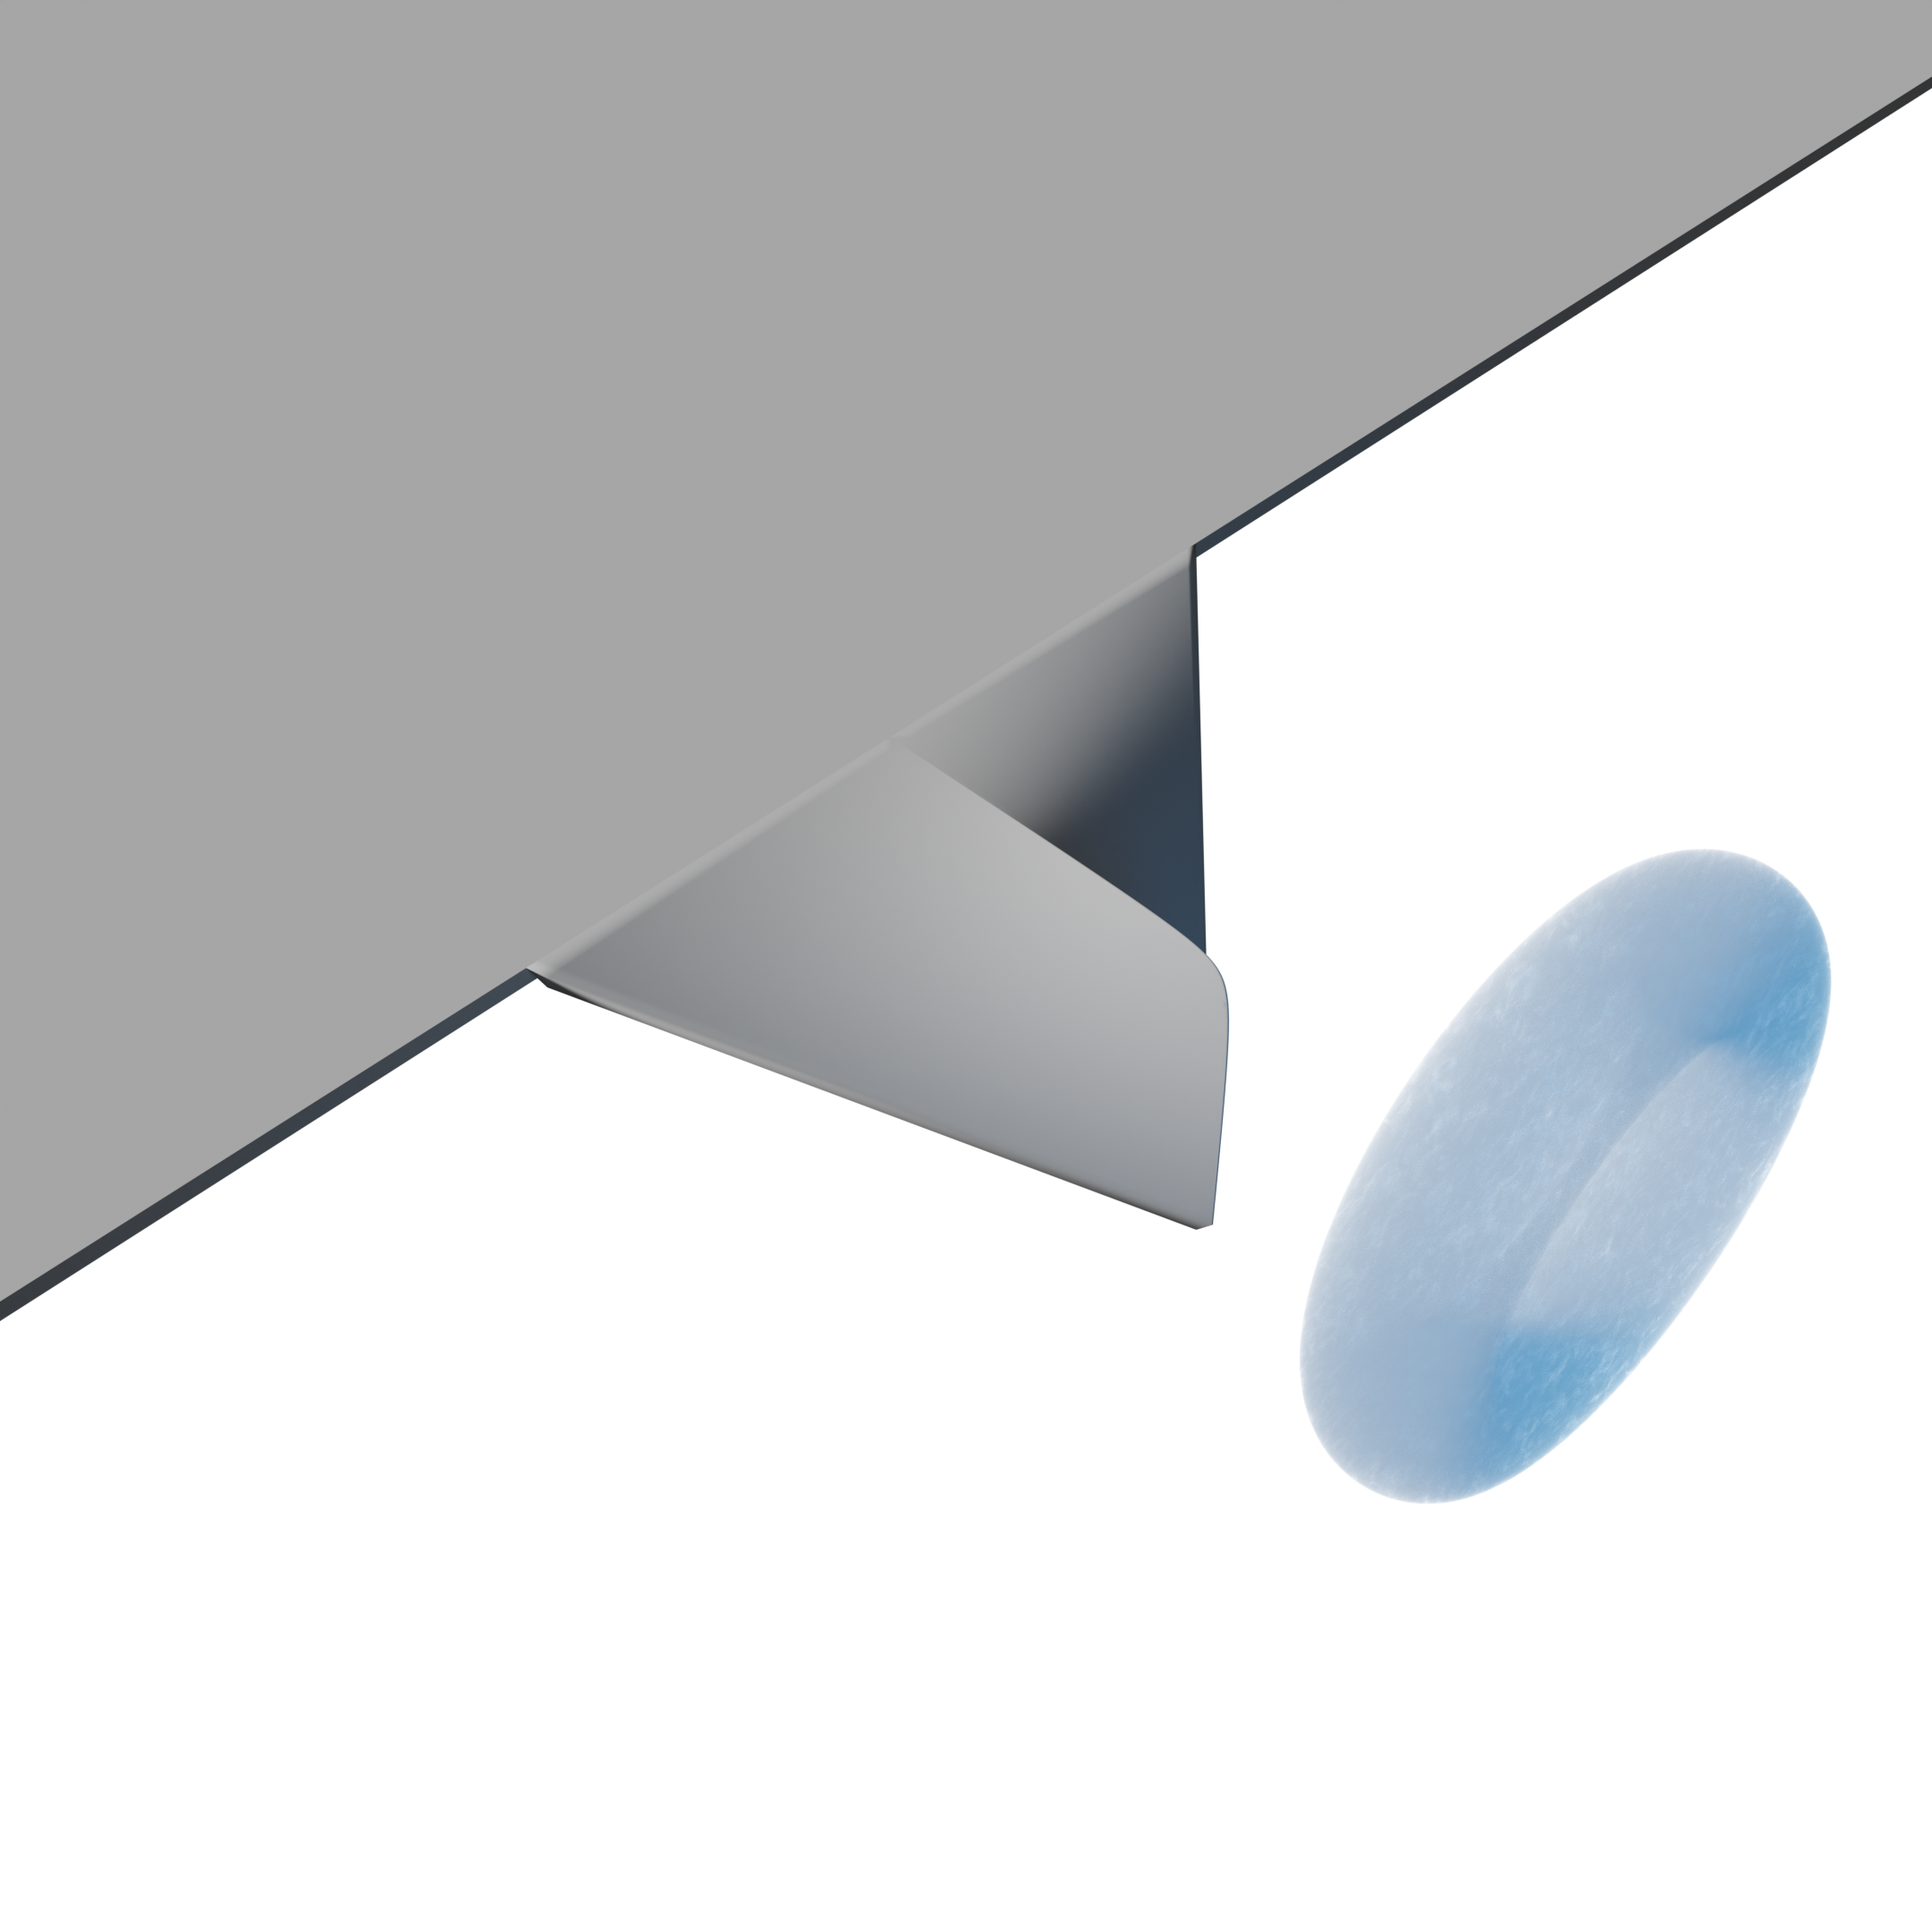
\includegraphics[width=0.3\textwidth]{papers/wirbelringe/fig/versuch_moment_1.png}
        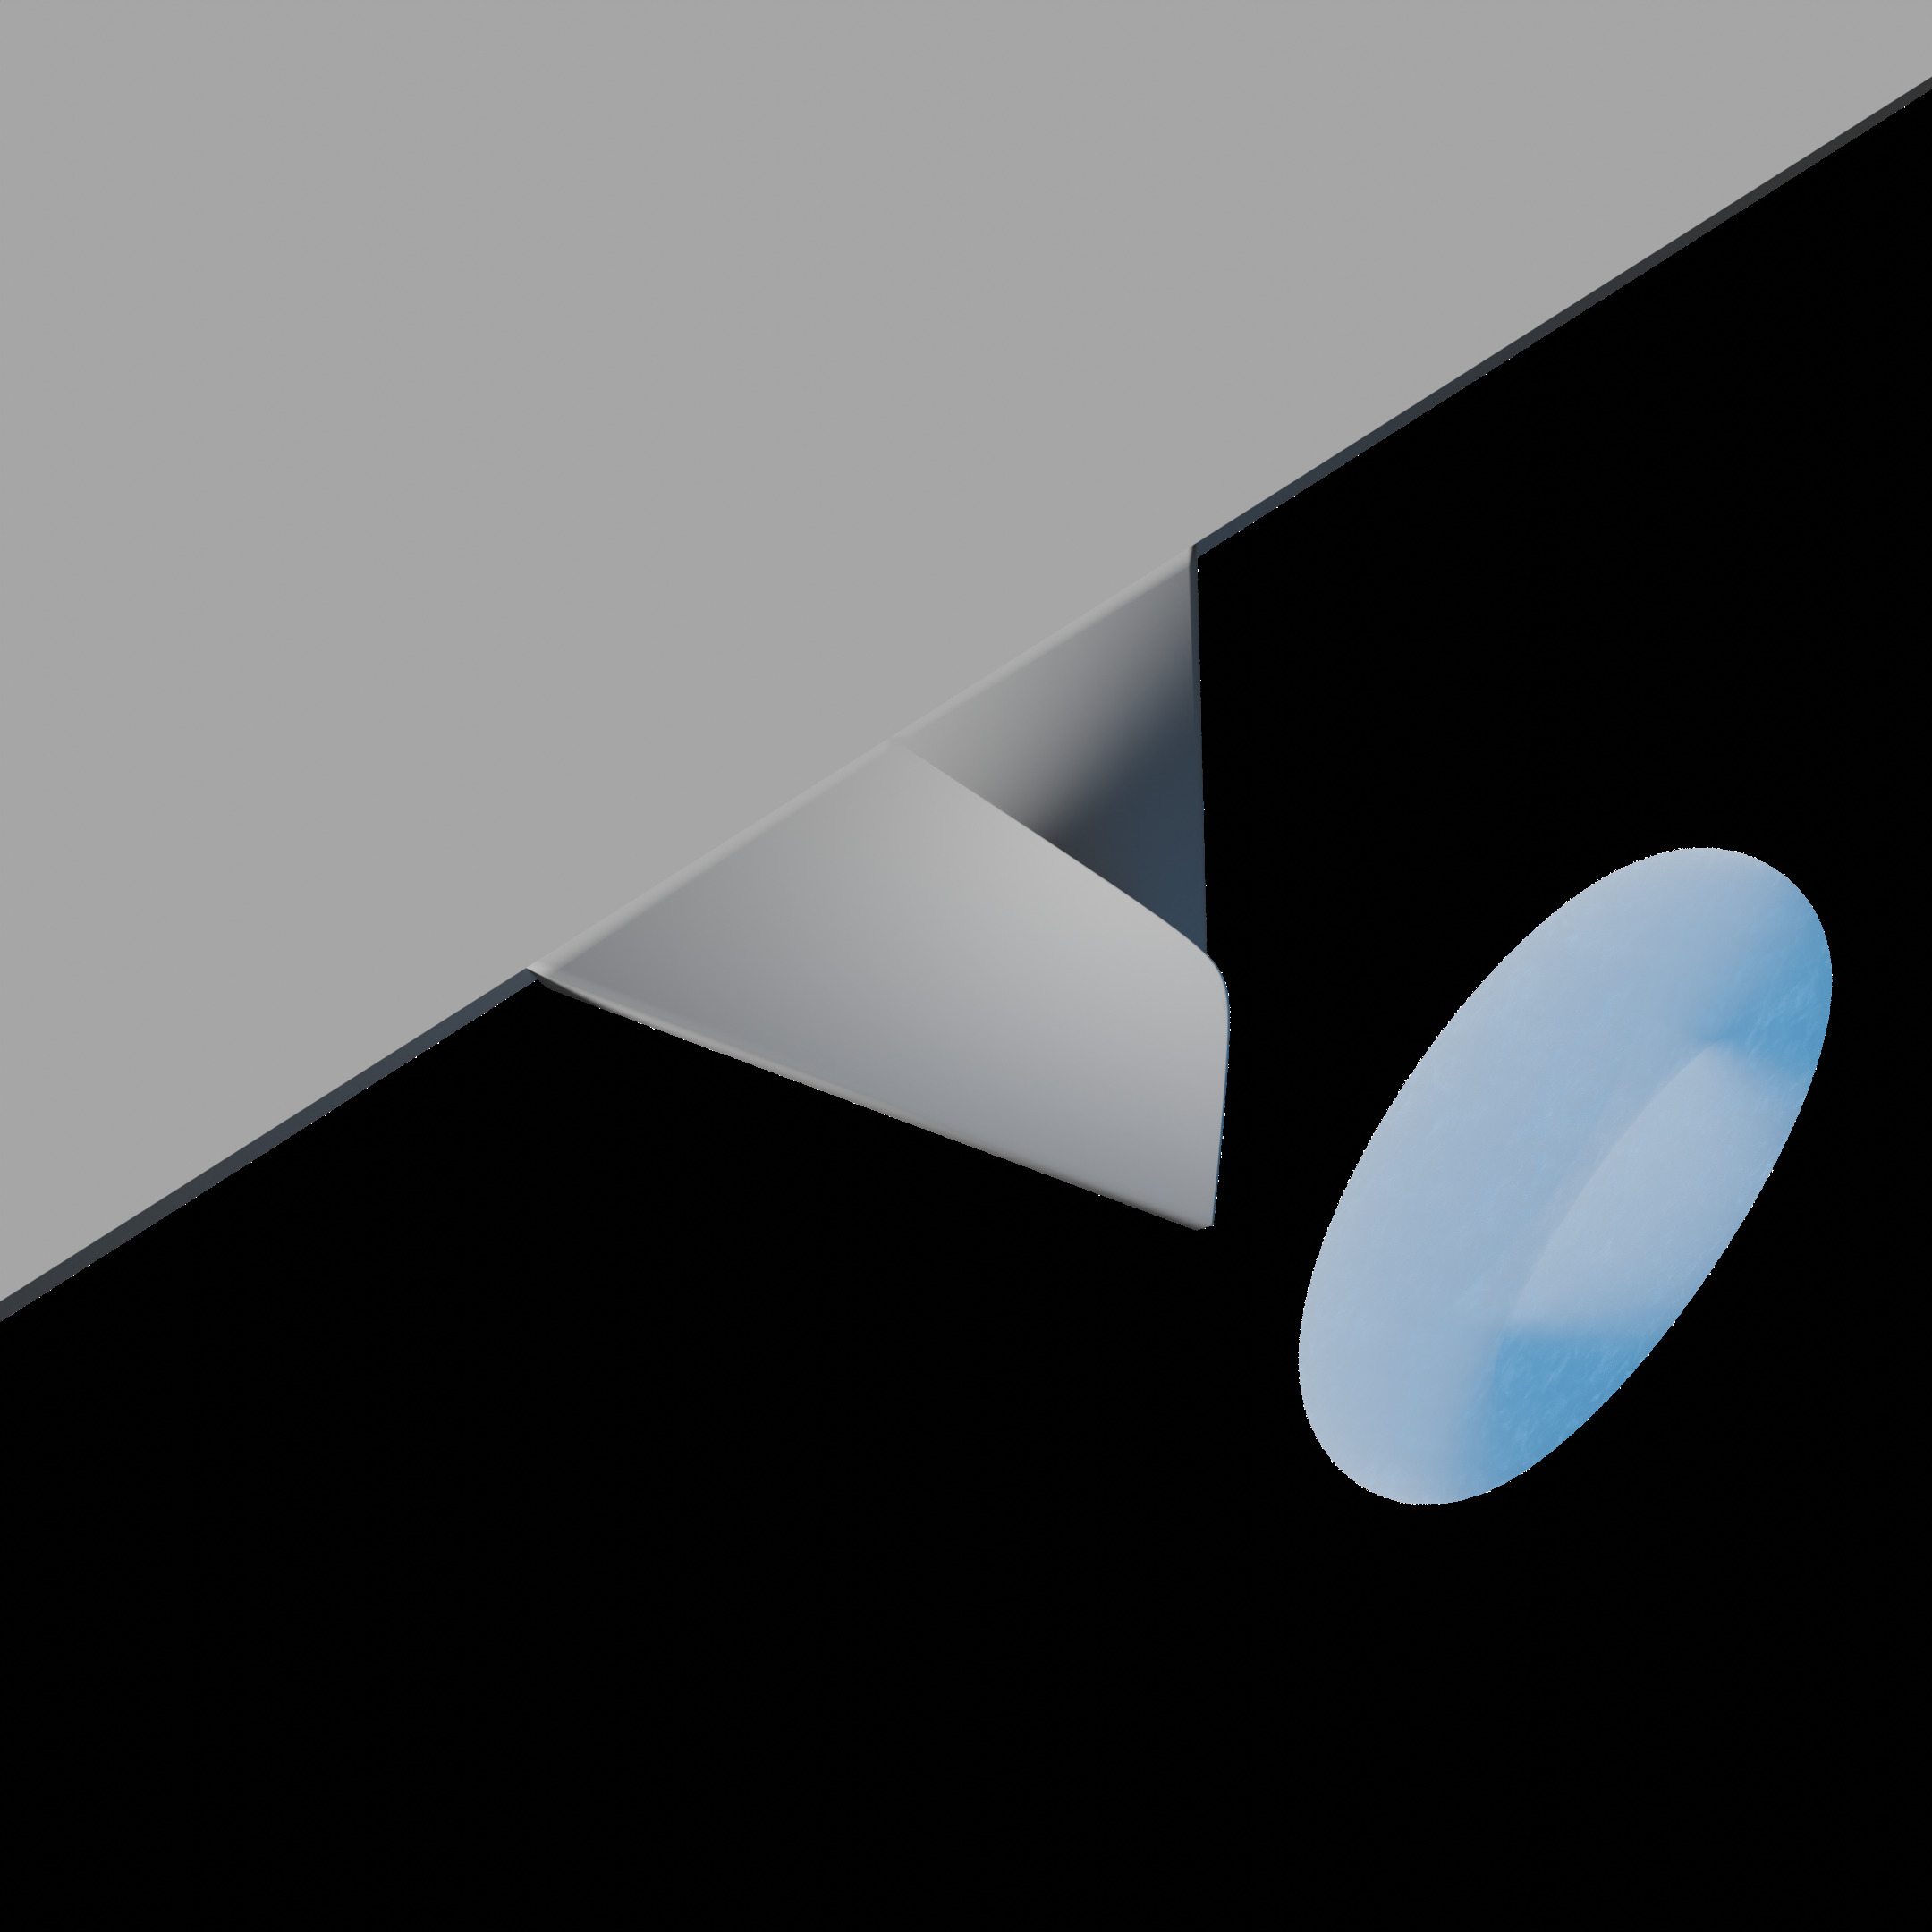
\includegraphics[width=0.3\textwidth]{papers/wirbelringe/fig/versuch_moment_1.jpg}
    }\hfill
    \subfigure[\label{Wirbelringe:fig:versuch_moment_2}]{
        %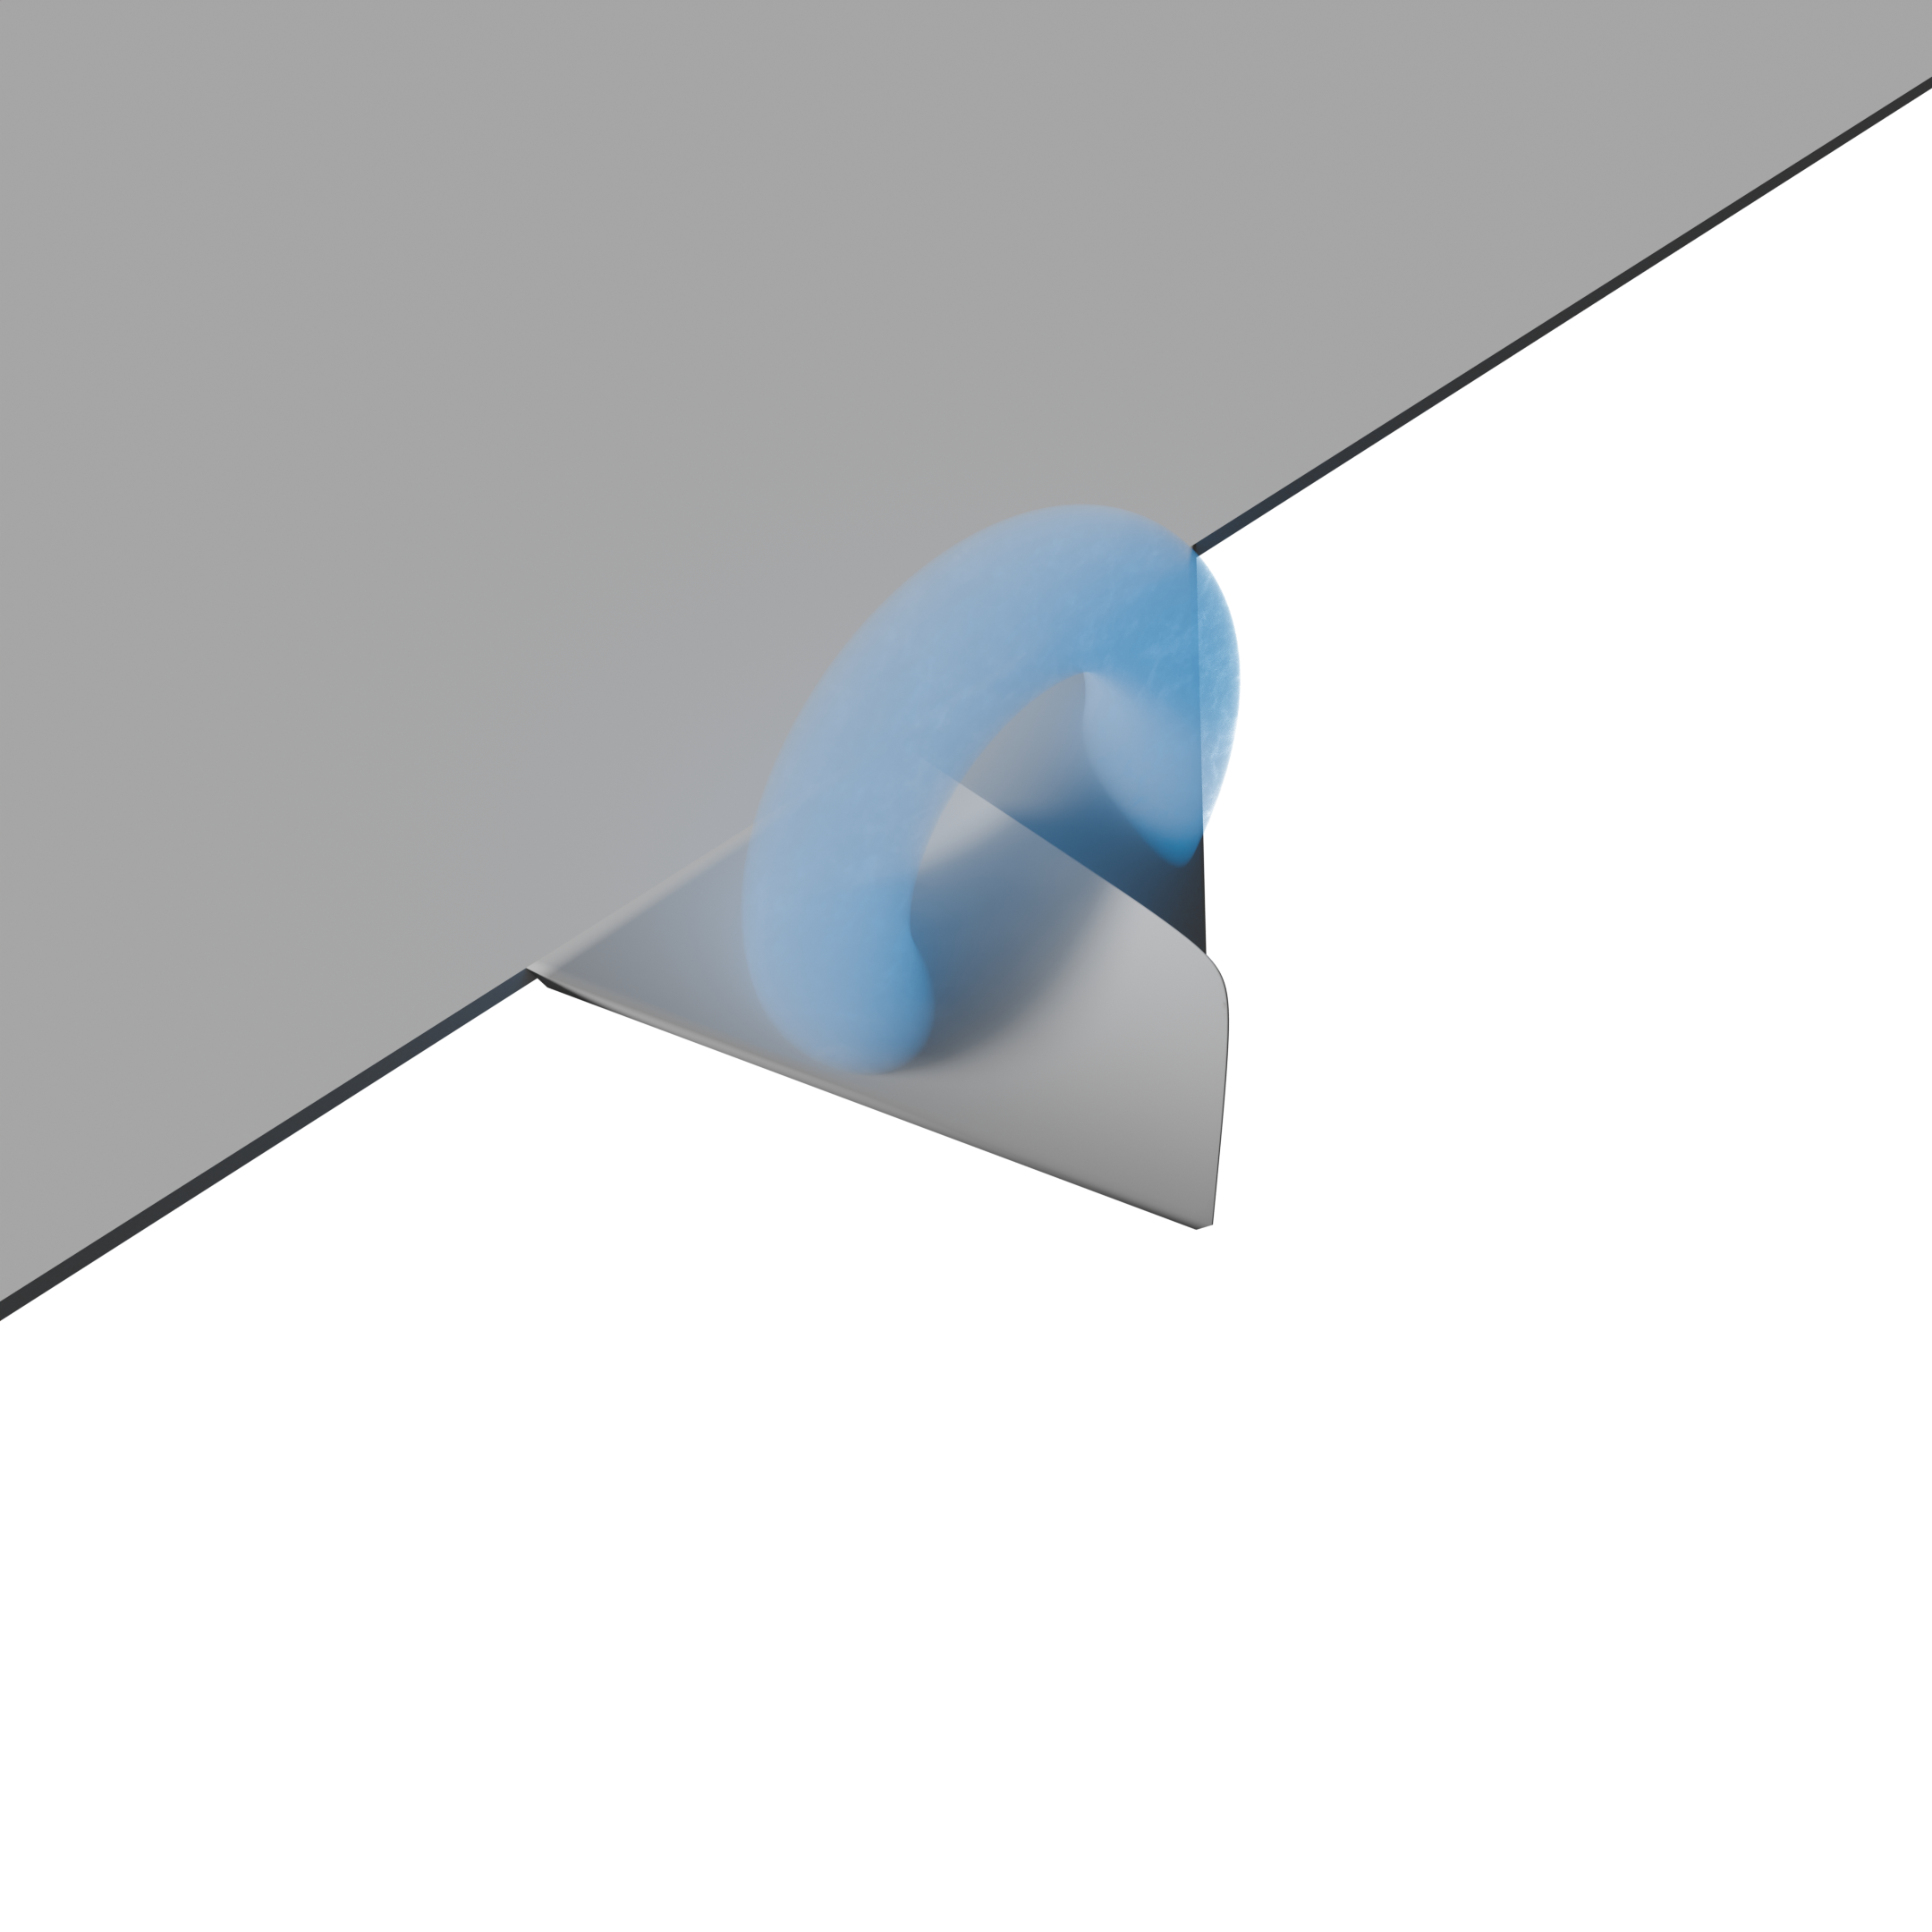
\includegraphics[width=0.3\textwidth]{papers/wirbelringe/fig/versuch_moment_2.png}
        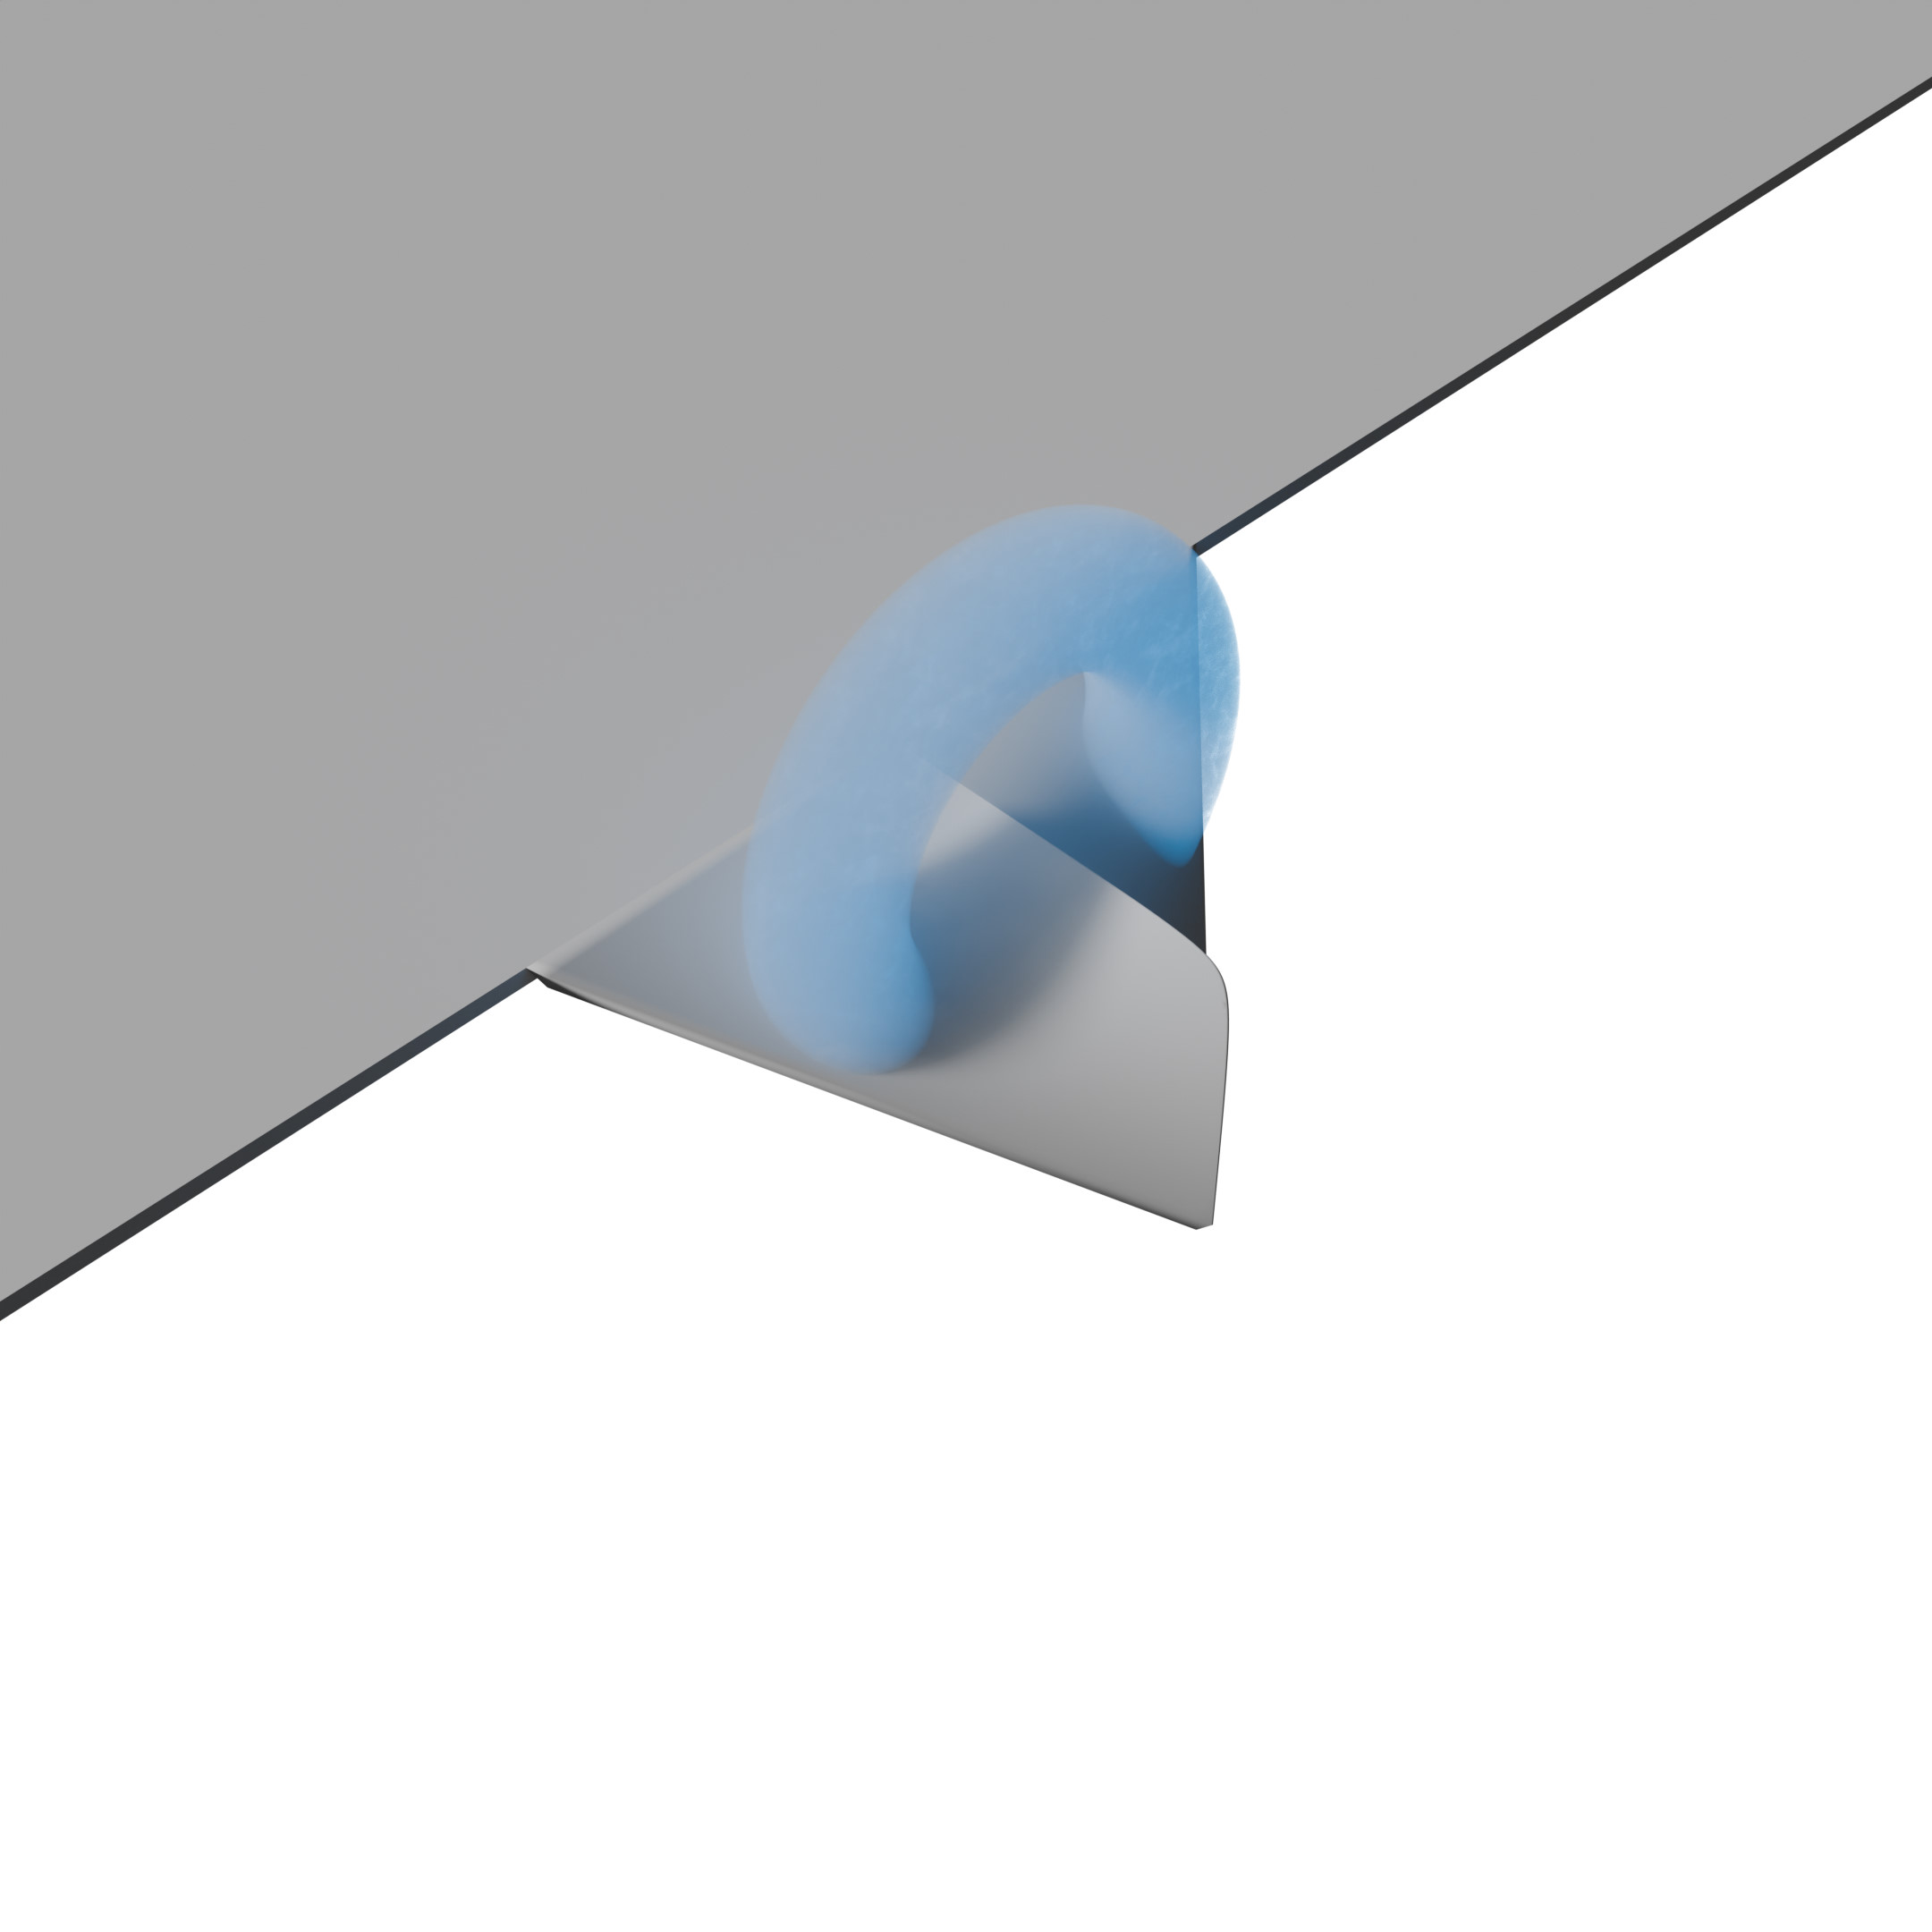
\includegraphics[width=0.3\textwidth]{papers/wirbelringe/fig/versuch_moment_2.jpg}
    }\hfill
    \subfigure[\label{Wirbelringe:fig:versuch_moment_3}]{
        %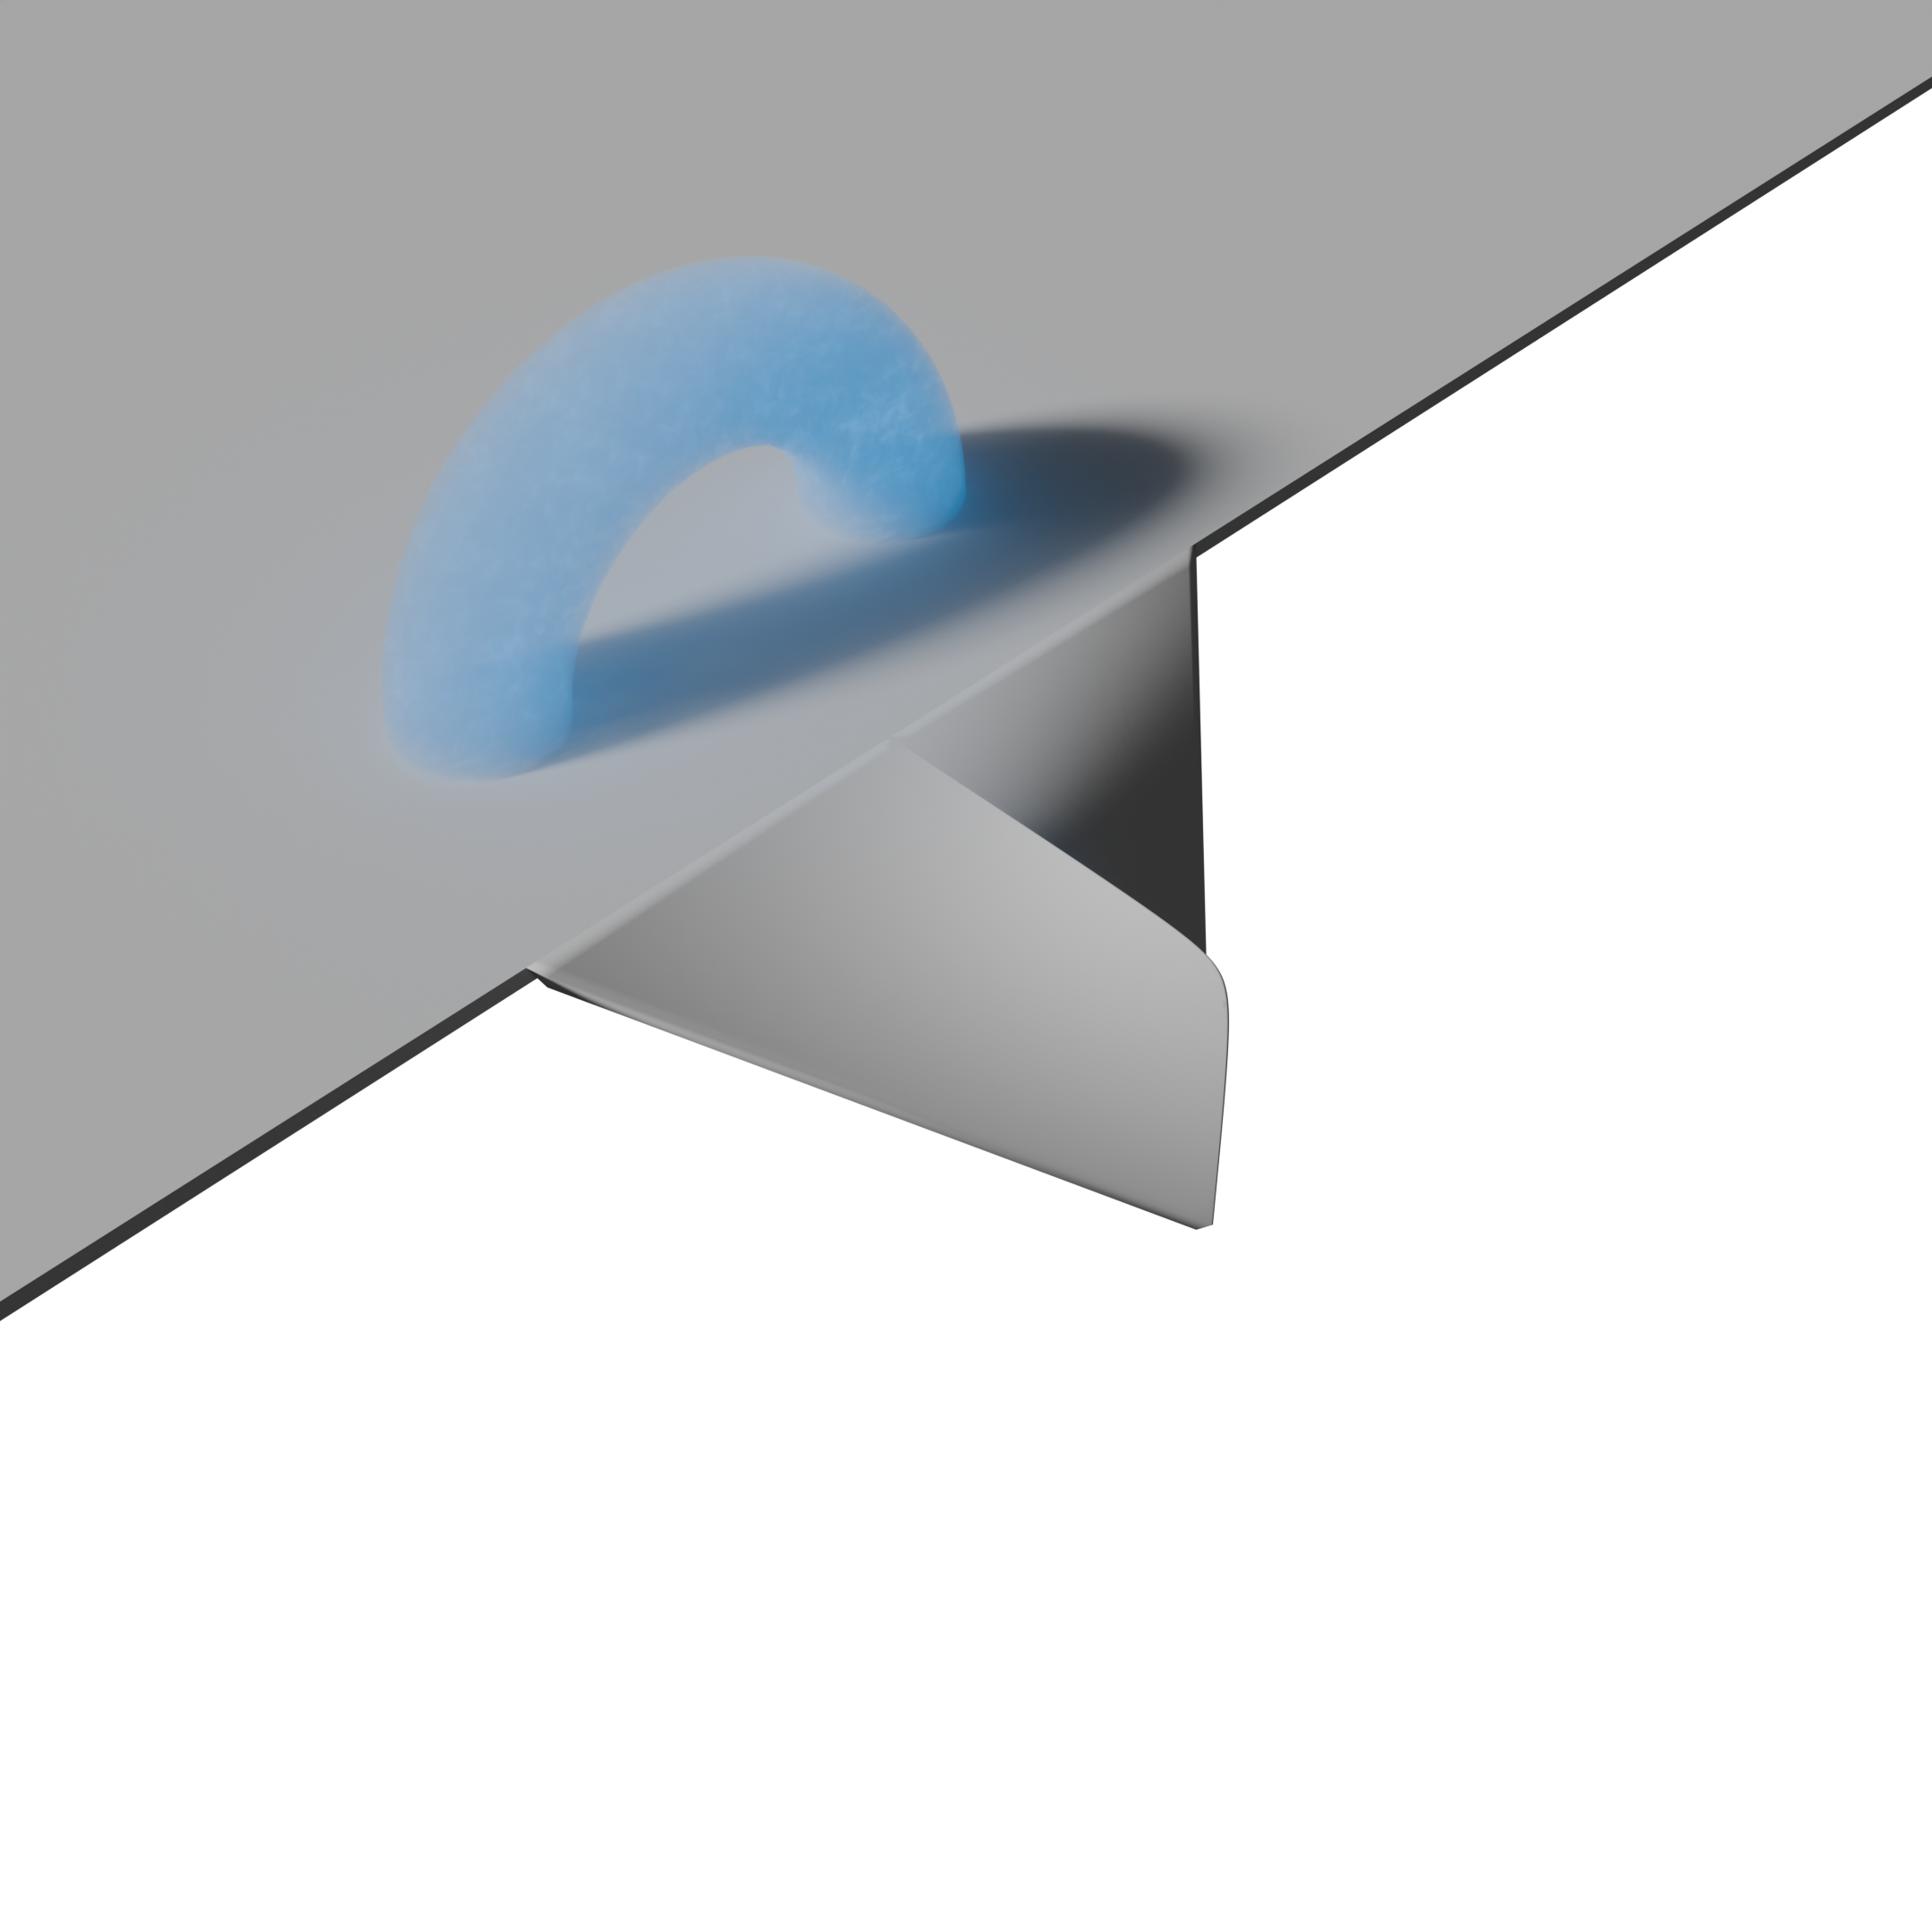
\includegraphics[width=0.3\textwidth]{papers/wirbelringe/fig/versuch_moment_3.png}
        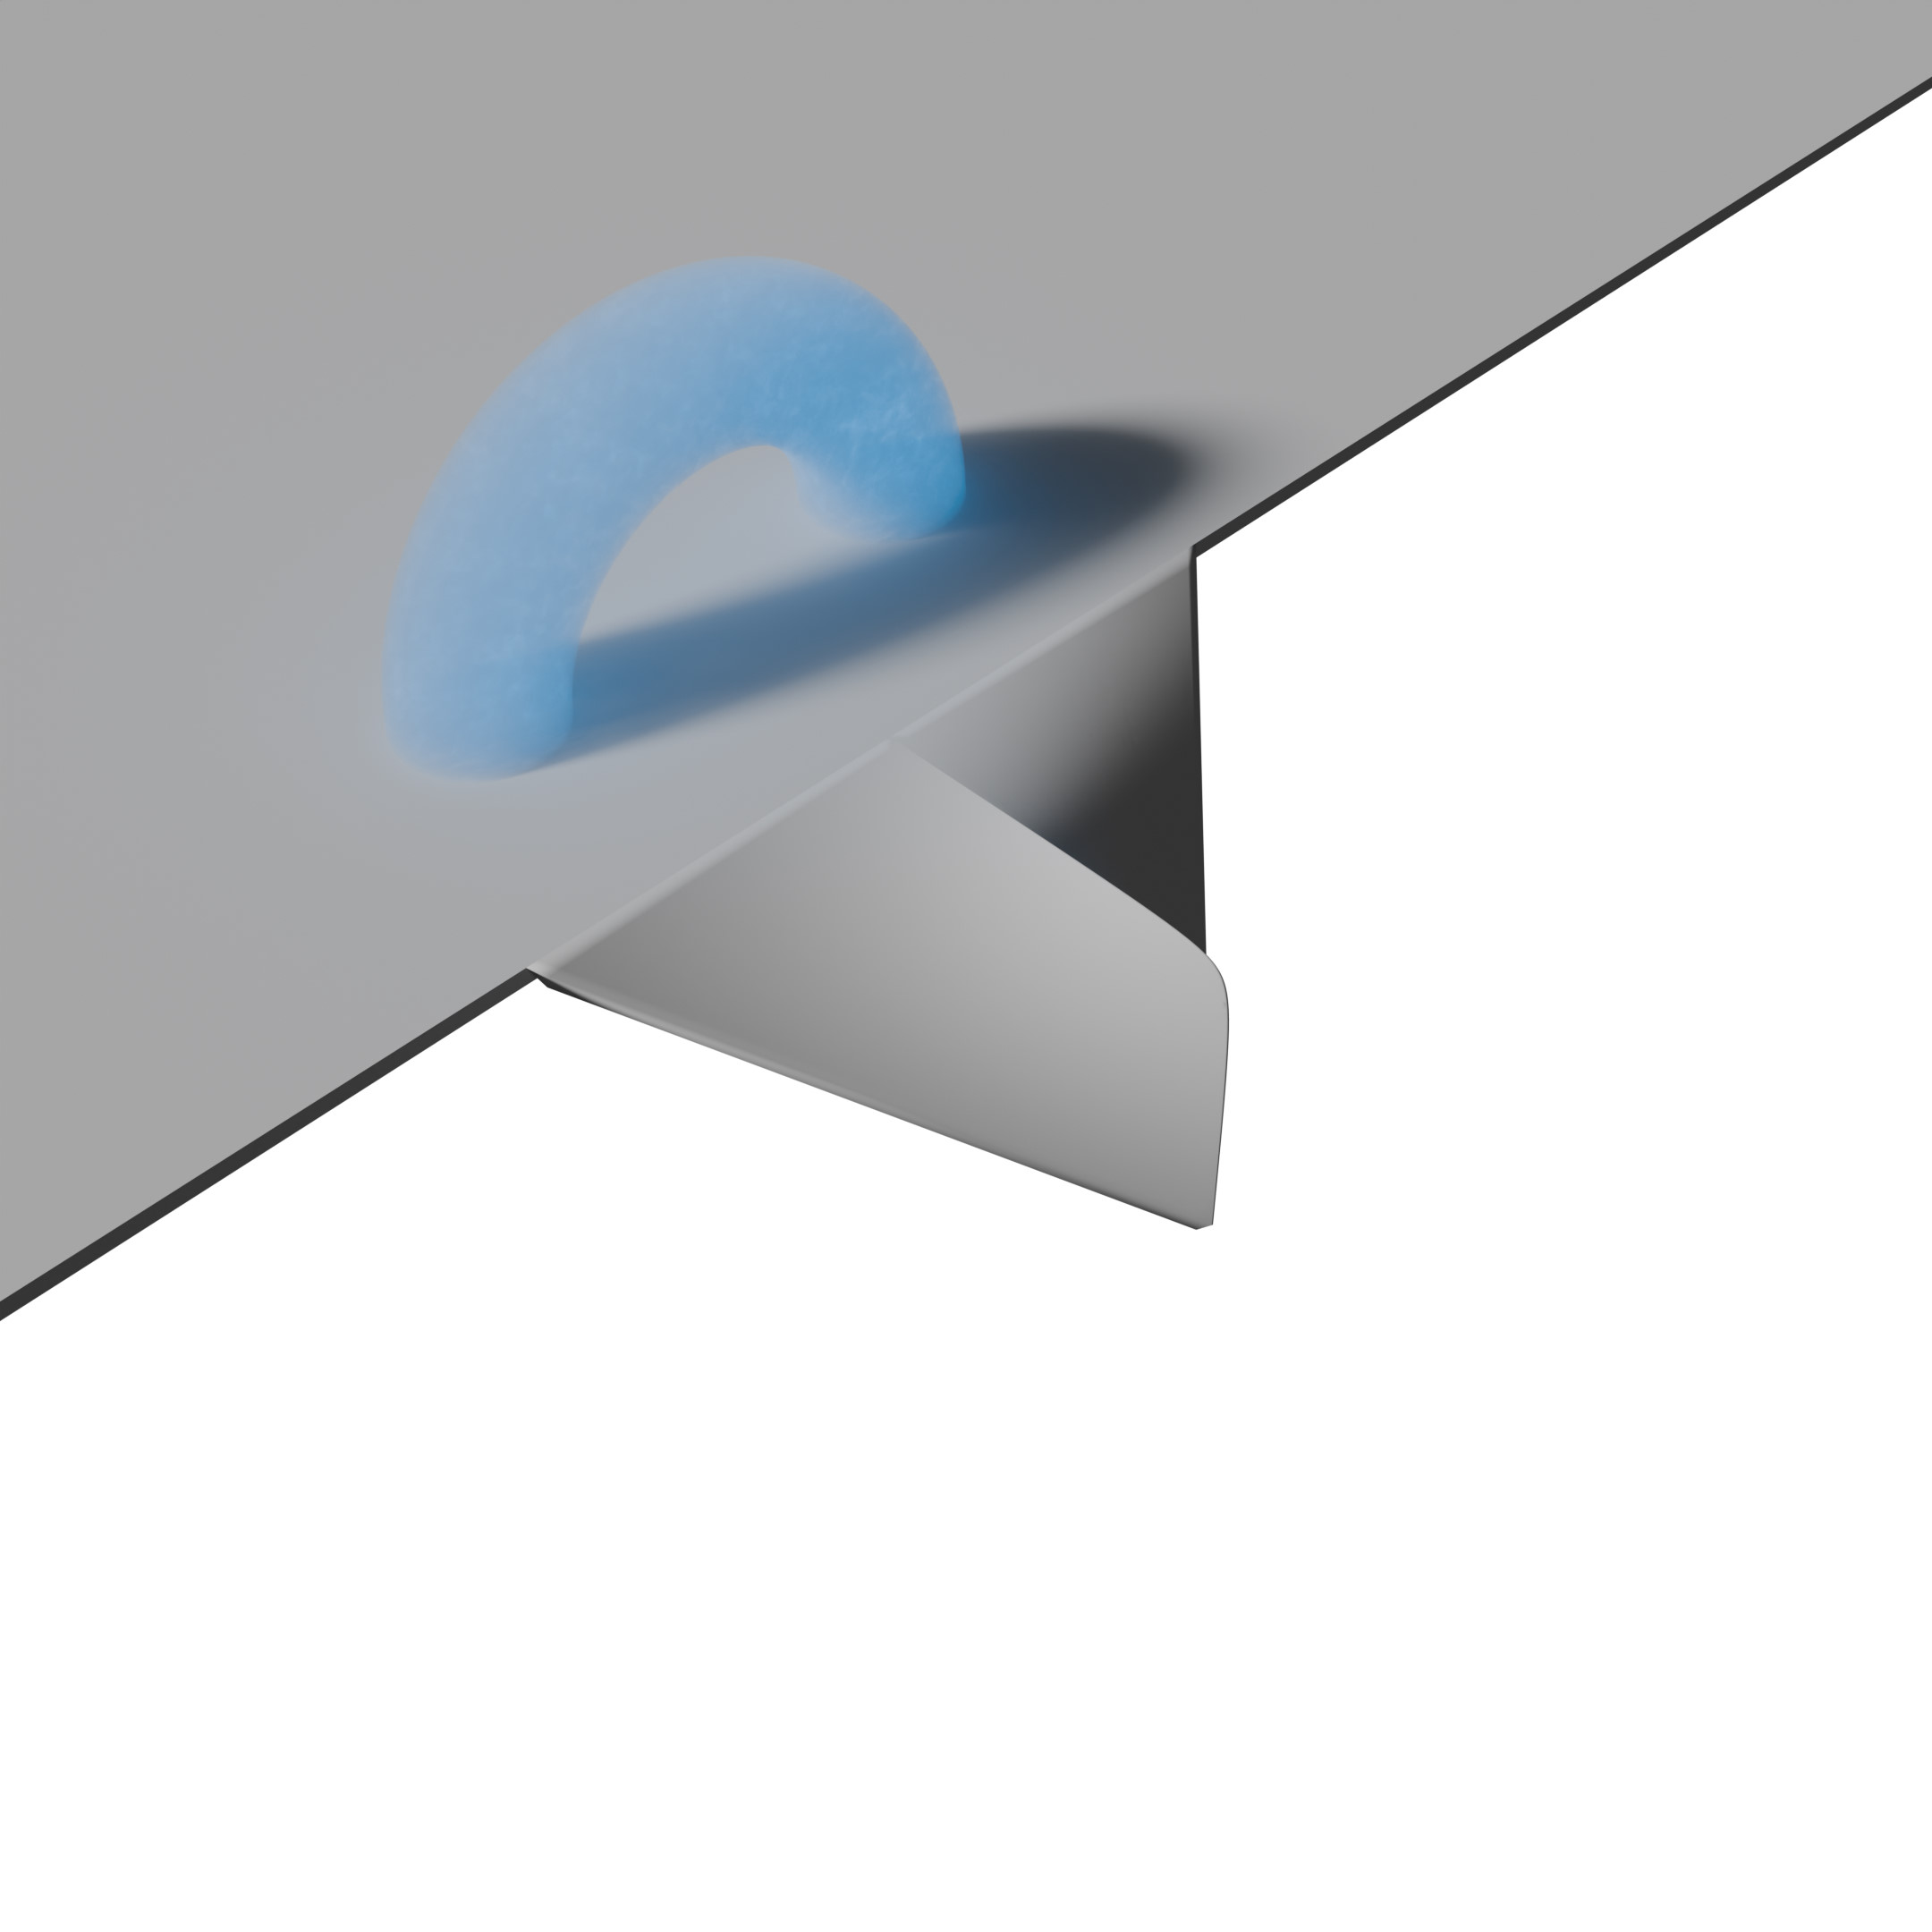
\includegraphics[width=0.3\textwidth]{papers/wirbelringe/fig/versuch_moment_3.jpg}
    }
    \caption{3D Darstellung in Blender des gewünschten Versuchsausgangs.}
    \label{Wirbelringe:fig:wirbelringversuch}
\end{figure}

